% answers.tex —— 2006 年·普通高等学校招生考试·湖北卷文科 · 参考答案与详细解析片段
% 由 tools/generate_projects.py 依来源总账自 2006/2006_数学真题_湖北文_试题.md + 2006/2006_数学真题_湖北文_解析正文.md + 2006/2006_数学真题_湖北文_答案要点.md 生成，勿手改（改源 MD 后重跑）
title: 2006 湖北卷文数学独立解析
year: 2006
source_id: src-af4cc84c7c2f6c2c1ed0bef598d5a51f57d65a1b25926d7a02631cc6c5387d75
source_sha256: b7de4b974a9d512908f6104f3acfdd3785328cd6a1a7ca7ea4578e2fa0d37379
paper_id: gk-2006-regular-hubei-arts
official_answer: null
solution_status: independently-derived-q12-pending
\par\medskip

\begin{gktip}
以下为依据固定候选题面独立求解的内容，不是官方答案或解析。固定 PDF 未见答案、解析或评分材料；来源发布者、出版者、版次与来源链未核。
\end{gktip}

\begin{answer}
\gksolhead{1}{}

\textbf{题目}：

集合 $P=\{x\mid x^2-16<0\}$，$Q=\{x\mid x=2n,\ n\in\mathbb Z\}$，则 $P\cap Q=$\mbox{（　　）}。

（A）$\{-2,\ 2\}$　　（B）$\{-2,\ 2,\ -4,\ 4\}$

（C）$\{-2,\ 0,\ 2\}$　　（D）$\{-2,\ 2,\ 0,\ -4,\ 4\}$

\Needspace{4\baselineskip}
\textbf{解析}

$P=(-4,4)$，而 $Q$ 为全体偶整数，故 $P\cap Q=\{-2,0,2\}$，选 C。

\gkanswer{答案：C}

\end{answer}
\begin{answer}
\gksolhead{2}{}

\textbf{题目}：

已知非零向量 $\vec a,\vec b$，若 $\vec a+2\vec b$ 与 $\vec a-2\vec b$ 互相垂直，则 $\dfrac{|\vec a|}{|\vec b|}=$\mbox{（　　）}。

（A）$\dfrac14$　　（B）$4$　　（C）$\dfrac12$　　（D）$2$

\Needspace{4\baselineskip}
\textbf{解析}

\Needspace{5\baselineskip}
由垂直条件，
\nopagebreak[4]
\[
(\vec a+2\vec b)\cdot(\vec a-2\vec b)=|\vec a|^2-4|\vec b|^2=0.
\]
因此 $|\vec a|/|\vec b|=2$，选 D。

\gkanswer{答案：D}

\end{answer}
\begin{answer}
\gksolhead{3}{}

\textbf{题目}：

已知 $\sin 2\alpha=\dfrac23$，$\alpha\in(0,\pi)$，则 $\sin\alpha+\cos\alpha=$\mbox{（　　）}。

（A）$\dfrac{\sqrt{15}}3$　　（B）$-\dfrac{\sqrt{15}}3$　　（C）$\dfrac53$　　（D）$-\dfrac53$

\Needspace{4\baselineskip}
\textbf{解析}

\Needspace{5\baselineskip}
$\alpha\in(0,\pi)$ 且 $\sin2\alpha>0$，所以 $\alpha\in(0,\pi/2)$，从而 $\sin\alpha+\cos\alpha>0$。于是
\nopagebreak[4]
\[
(\sin\alpha+\cos\alpha)^2=1+\sin2\alpha=\frac53,
\]
故所求为 $\sqrt{15}/3$，选 A。

\gkanswer{答案：A}

\end{answer}
\begin{answer}
\gksolhead{4}{}

\textbf{题目}：

在等比数列 $\{a_n\}$ 中，$a_1=1$，$a_{10}=3$，则 $a_2a_3a_4a_5a_6a_7a_8a_9=$\mbox{（　　）}。

（A）$81$　　（B）$27\sqrt[5]{27}$　　（C）$\sqrt3$　　（D）$243$

\Needspace{4\baselineskip}
\textbf{解析}

\Needspace{5\baselineskip}
设公比为 $q$，则 $q^9=a_{10}/a_1=3$。所以
\nopagebreak[4]
\[
a_2a_3\cdots a_9=q^{1+2+\cdots+8}=q^{36}=(q^9)^4=81,
\]
选 A。

\gkanswer{答案：A}

\end{answer}
\begin{answer}
\gksolhead{5}{}

\textbf{题目}：

甲：$A_1\text{、}A_2$ 是互斥事件；乙：$A_1\text{、}A_2$ 是对立事件。那么\mbox{（　　）}。

（A）甲是乙的充分条件但不是必要条件

（B）甲是乙的必要条件但不是充分条件

（C）甲是乙的充要条件

（D）甲既不是乙的充分条件，也不是乙的必要条件

\Needspace{4\baselineskip}
\textbf{解析}

对立事件必互斥；互斥事件未必覆盖整个样本空间。因此“甲是乙的必要条件但不是充分条件”，选 B。

\gkanswer{答案：B}

\end{answer}
\begin{answer}
\gksolhead{6}{}

\textbf{题目}：

关于直线 $m,n$ 与平面 $\alpha,\beta$，有以下四个命题：

① 若 $m\parallel\alpha$，$n\parallel\beta$ 且 $\alpha\parallel\beta$，则 $m\parallel n$；

② 若 $m\perp\alpha$，$n\perp\beta$ 且 $\alpha\perp\beta$，则 $m\perp n$；

③ 若 $m\perp\alpha$，$n\parallel\beta$ 且 $\alpha\parallel\beta$，则 $m\perp n$；

④ 若 $m\parallel\alpha$，$n\perp\beta$ 且 $\alpha\perp\beta$，则 $m\parallel n$。

其中真命题的序号是\mbox{（　　）}。

（A）①②　　（B）③④　　（C）①④　　（D）②③

\Needspace{4\baselineskip}
\textbf{解析}

①两平面平行时，分别平行于这两个平面的直线方向未必相同，假；②两直线分别沿两互相垂直平面的法向，故互相垂直，真；③$\alpha\parallel\beta$ 且 $n\parallel\beta$，所以 $n$ 的方向平行于 $\alpha$，而 $m\perp\alpha$，故 $m\perp n$，真；④$\alpha\perp\beta$ 只说明 $n$ 的方向平行于 $\alpha$，不能推出 $m\parallel n$，假。选 D（②③）。

\gkanswer{答案：D}

\end{answer}
\begin{answer}
\gksolhead{7}{}

\textbf{题目}：

设 $f(x)=\lg\dfrac{2+x}{2-x}$，则 $f\left(\dfrac{x}{2}\right)+f\left(\dfrac{2}{x}\right)$ 的定义域为\mbox{（　　）}。

（A）$(-4,0)\cup(0,4)$　　（B）$(-4,-1)\cup(1,4)$

（C）$(-2,-1)\cup(1,2)$　　（D）$(-4,-2)\cup(2,4)$

\Needspace{4\baselineskip}
\textbf{解析}

对 $f(u)$，真数为正等价于 $-2<u<2$。故 $f(x/2)$ 要求 $-4<x<4$；$f(2/x)$ 要求 $x\ne0$ 且 $|2/x|<2$，即 $x<-1$ 或 $x>1$。取交集得 $(-4,-1)\cup(1,4)$，选 B。

\gkanswer{答案：B}

\end{answer}
\begin{answer}
\gksolhead{8}{}

\textbf{题目}：

在 $\left(\sqrt{x}-\dfrac{1}{\sqrt[3]{x}}\right)^{24}$ 的展开式中，$x$ 的幂的指数是整数的项共有\mbox{（　　）}。

（A）3项　　（B）4项　　（C）5项　　（D）9项

\Needspace{4\baselineskip}
\textbf{解析}

\Needspace{5\baselineskip}
令通项中第二项的选取次数为 $k$，则 $x$ 的指数为
\nopagebreak[4]
\[
\frac{24-k}{2}-\frac{k}{3}=12-\frac{5k}{6},\qquad k=0,1,\ldots,24.
\]
指数为整数当且仅当 $k$ 为6的倍数，共有 $k=0,6,12,18,24$ 五项，选 C。

\gkanswer{答案：C}

\end{answer}
\begin{answer}
\gksolhead{9}{}

\textbf{题目}：

设过点 $P(x,y)$ 的直线分别与 $x$ 轴的正半轴和 $y$ 轴的正半轴交于 $A,B$ 两点，点 $Q$ 与点 $P$ 关于 $y$ 轴对称，$O$ 为坐标原点，若 $\overrightarrow{BP}=2\overrightarrow{PA}$ 且 $\overrightarrow{OQ}\cdot\overrightarrow{AB}=1$，则点 $P$ 的轨迹方程是\mbox{（　　）}。

（A）$3x^2+\dfrac32y^2=1\ (x>0,\ y>0)$　　（B）$3x^2-\dfrac32y^2=1\ (x>0,\ y>0)$

（C）$\dfrac32x^2-3y^2=1\ (x>0,\ y>0)$　　（D）$\dfrac32x^2+3y^2=1\ (x>0,\ y>0)$

\Needspace{4\baselineskip}
\textbf{解析}

\Needspace{5\baselineskip}
设 $A=(a,0)$、$B=(0,b)$、$P=(x,y)$。由 $\overrightarrow{BP}=2\overrightarrow{PA}$ 得 $P-B=2(A-P)$，故 $a=3x/2$、$b=3y$。又 $Q=(-x,y)$，所以
\nopagebreak[4]
\[
\overrightarrow{OQ}\cdot\overrightarrow{AB}=(-x,y)\cdot(-a,b)=xa+yb=\frac32x^2+3y^2=1.
\]
这对应选项 D。

\gkanswer{答案：D}

\end{answer}
\begin{answer}
\gksolhead{10}{}

\textbf{题目}：

关于 $x$ 的方程 $(x^2-1)^2-|x^2-1|+k=0$，给出下列四个命题：

① 存在实数 $k$，使得方程恰有2个不同的实根；

② 存在实数 $k$，使得方程恰有4个不同的实根；

③ 存在实数 $k$，使得方程恰有5个不同的实根；

④ 存在实数 $k$，使得方程恰有8个不同的实根。

其中假命题的个数是\mbox{（　　）}。

（A）0　　（B）1　　（C）2　　（D）3

\Needspace{4\baselineskip}
\textbf{解析}

令 $u=|x^2-1|\geqslant0$，方程化为 $u^2-u+k=0$。取 $k<0$ 可得到2个不同实根；取 $k=1/4$ 得到4个；取 $k=0$ 得到5个；取 $0<k<1/4$ 时有两个不同的正 $u$，各对应4个 $x$，共8个。四个存在性命题都为真，假命题数为0，选 A。

\gkanswer{答案：A}

\end{answer}
\begin{answer}
\gksolhead{11}{}

\textbf{题目}：

在 $\triangle ABC$ 中，已知 $a=\dfrac{4\sqrt3}{3}$，$b=4$，$A=30^\circ$，则 $\sin B=$\gkblank{}。

\Needspace{4\baselineskip}
\textbf{解析}

\Needspace{5\baselineskip}
由正弦定理，
\nopagebreak[4]
\[
\sin B=\frac{b\sin A}{a}
=\frac{4\cdot\frac12}{4\sqrt3/3}
=\frac{\sqrt3}{2}.
\]
SSA 条件可能使 $B$ 为 $60^\circ$ 或 $120^\circ$，但两种情形的正弦相同，所以所问值唯一。

\gkanswer{答案：$\dfrac{\sqrt3}{2}$}

\end{answer}
\begin{answer}
\gksolhead{12}{}

\textbf{题目}：

接种某疫苗后，出现发热反应的概率为 $0.80$，现有5人接种该疫苗，至少有3人出现发热反应的概率为\gkblank{}。（精确到0.01）

\Needspace{4\baselineskip}
\textbf{解析}

\Needspace{5\baselineskip}
固定题面只给出每人的边缘概率 $0.8$，没有声明五人的反应相互独立。若五人反应完全同动（每人仍各有 $0.8$ 的概率发热），至少3人发热的概率为 $0.8$；若五人相互独立，则
\nopagebreak[4]
\[
P(X\geqslant3)=\binom53(0.8)^3(0.2)^2+\binom54(0.8)^4(0.2)+(0.8)^5=0.94208,
\]
精确到0.01为 $0.94$。不同联合模型给出不同结果，因此按固定题面本身保留 U/PENDING；$0.94$ 仅为独立假设下的条件计算。

\gkanswer{答案：U/PENDING；仅按题面给出的边缘概率不能确定联合事件概率。若五人反应相互独立，条件答案为 $0.94$}

\end{answer}
\begin{answer}
\gksolhead{13}{}

\textbf{题目}：

若直线 $y=kx+2$ 与圆 $(x-2)^2+(y-3)^2=1$ 有两个不同的交点，则 $k$ 的取值范围是\gkblank{}。

\Needspace{4\baselineskip}
\textbf{解析}

\Needspace{5\baselineskip}
圆心 $(2,3)$ 到直线 $kx-y+2=0$ 的距离小于半径1：
\nopagebreak[4]
\[
\frac{|2k-1|}{\sqrt{k^2+1}}<1
\iff (2k-1)^2<k^2+1
\iff 3k^2-4k<0.
\]
故 $0<k<4/3$。

\gkanswer{答案：$0<k<\dfrac43$}

\end{answer}
\begin{answer}
\gksolhead{14}{}

\textbf{题目}：

安排5名歌手的演出顺序时，要求某名歌手不第一个出场，另一名歌手不最后一个出场，不同排法的总数是\gkblank{}。（用数字作答）

\Needspace{4\baselineskip}
\textbf{解析}

\Needspace{5\baselineskip}
从全部 $5!$ 种排列中，减去指定歌手排第一的 $4!$ 种及另一指定歌手排最后的 $4!$ 种，再加回两者同时发生的 $3!$ 种，得
\nopagebreak[4]
\[
5!-4!-4!+3!=78.
\]

\gkanswer{答案：$78$}

\end{answer}
\begin{answer}
\gksolhead{15}{}

\textbf{题目}：

半径为 $r$ 的圆的面积 $S(r)=\pi r^2$，周长 $C(r)=2\pi r$，若将 $r$ 看作 $(0,+\infty)$ 上的变量，则 $(\pi r^2)'=2\pi r$ ①，①式可以用语言叙述为：圆的面积函数的导数等于圆的周长函数。对于半径为 $R$ 的球，若将 $R$ 看作 $(0,+\infty)$ 上的变量，请你写出类似于①的式子：\gkblank{}②，②式可以用语言叙述为：\gkblank{}。

\Needspace{4\baselineskip}
\textbf{解析}

\Needspace{5\baselineskip}
球的体积函数为 $V(R)=\dfrac43\pi R^3$，因此
\nopagebreak[4]
\[
V'(R)=\left(\frac43\pi R^3\right)'=4\pi R^2.
\]
右端是球的表面积函数，故语言表述为：球的体积函数的导数等于球的表面积函数。

\gkanswer{答案：$\left(\dfrac43\pi R^3\right)'=4\pi R^2$；球的体积函数的导数等于球的表面积函数}

\end{answer}
\begin{answer}
\gksolhead{16}{}

\textbf{题目}：

设向量 $\vec a=(\sin x,\cos x)$，$\vec b=(\cos x,\cos x)$，$x\in\mathbb R$，函数 $f(x)=\vec a\cdot(\vec a+\vec b)$。

（1） 求函数 $f(x)$ 的最大值与最小正周期；

（2） 求使不等式 $f(x)\geqslant\dfrac32$ 成立的 $x$ 的取值集。

\Needspace{4\baselineskip}
\textbf{解析}

\textbf{（1）}

\Needspace{5\baselineskip}
由向量点积，
\nopagebreak[4]
\[
f(x)=\sin^2x+\sin x\cos x+2\cos^2x
=\frac32+\frac12(\cos2x+\sin2x)
=\frac32+\frac{\sqrt2}{2}\cos\left(2x-\frac\pi4\right).
\]
所以最大值为 $(3+\sqrt2)/2$，最小正周期为 $\pi$。

\textbf{（2）}

\Needspace{5\baselineskip}
不等式 $f(x)\geqslant3/2$ 等价于 $\cos(2x-\pi/4)\geqslant0$，故
\nopagebreak[4]
\[
x\in\left[-\frac\pi8+k\pi,\frac{3\pi}8+k\pi\right],\qquad k\in\mathbb Z.
\]

\gkanswer{答案（1）：最大值 $\dfrac{3+\sqrt2}{2}$，最小正周期 $\pi$}

\gkanswer{答案（2）：$x\in[-\dfrac\pi8+k\pi,\dfrac{3\pi}8+k\pi]$，$k\in\mathbb Z$}

\end{answer}
\begin{answer}
\gksolhead{17}{}

\textbf{题目}：

某单位最近组织了一次健身活动，活动分为登山组和游泳组，且每个职工至多参加了其中一组。在参加活动的职工中，青年人占 $42.5\%$，中年人占 $47.5\%$，老年人占 $10\%$。登山组的职工占参加活动总人数的 $\dfrac14$，且该组中，青年人占 $50\%$，中年人占 $40\%$，老年人占 $10\%$。为了了解各组不同年龄层次的职工对本次活动的满意程度，现用分层抽样的方法从参加活动的全体职工中抽取一个容量为200的样本。试确定：

（1） 游泳组中，青年人、中年人、老年人分别所占的比例；

（2） 游泳组中，青年人、中年人、老年人分别应抽取的人数。

\Needspace{4\baselineskip}
\textbf{解析}

\textbf{（1）}

\Needspace{5\baselineskip}
以参加活动职工总人数为1，登山组中三年龄层占全体的比例依次为
\nopagebreak[4]
\[
\frac14\left(\frac12,\frac25,\frac1{10}\right)=\left(\frac18,\frac1{10},\frac1{40}\right).
\]
\Needspace{5\baselineskip}
游泳组中三年龄层占全体的比例为
\nopagebreak[4]
\[
\left(\frac{17}{40},\frac{19}{40},\frac1{10}\right)
-\left(\frac18,\frac1{10},\frac1{40}\right)
=\left(\frac3{10},\frac38,\frac3{40}\right),
\]
游泳组总比例为 $3/4$，故组内年龄比例为 $40\%\text{、}50\%\text{、}10\%$。

\textbf{（2）}

\Needspace{5\baselineskip}
总样本按全体年龄层分层抽取时，游泳组对应人数为
\nopagebreak[4]
\[
200\left(\frac3{10},\frac38,\frac3{40}\right)=(60,75,15).
\]

\gkanswer{答案（1）：青年人40\%，中年人50\%，老年人10\%}

\gkanswer{答案（2）：青年人60人，中年人75人，老年人15人}

\end{answer}
\begin{answer}
\gksolhead{18}{}

\textbf{题目}：

如图，已知正三棱柱 $ABC-A_1B_1C_1$ 的侧棱长和底面边长均为1，$M$ 是底面 $BC$ 边上的中点，$N$ 是侧棱 $CC_1$ 上的点，且 $CN=2C_1N$。
\nopagebreak[4]
\begin{center}% Source: 2006湖北文.pdf, source-relative PDF page 1, Q18.
% Non-scale vector redraw; solid/dashed visibility follows the fixed candidate image.
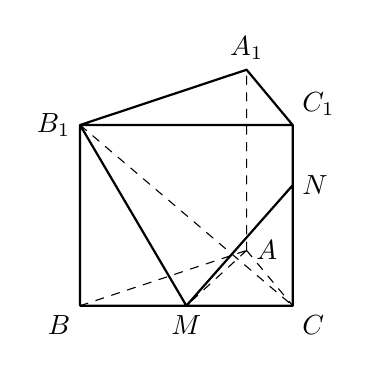
\begin{tikzpicture}[line cap=round,line join=round,x=0.9cm,y=0.9cm]
  \coordinate (B)  at (0,0);
  \coordinate (C)  at (3,0);
  \coordinate (M)  at (1.5,0);
  \coordinate (A)  at (2.35,0.78);
  \coordinate (B1) at (0,2.55);
  \coordinate (C1) at (3,2.55);
  \coordinate (N)  at (3,1.70);
  \coordinate (A1) at (2.35,3.33);

  % Hidden/inner lines visible dashed in the source drawing.
  \draw[dashed] (B)--(A) (A)--(C) (A)--(A1) (B1)--(C) (A)--(M);

  % Prism edges and the two solid segments through M shown in the source.
  \draw[thick] (B)--(C) (B)--(B1) (B1)--(C1) (C)--(C1)
    (B1)--(A1)--(C1) (B1)--(M) (M)--(N);

  \node[below left] at (B) {$B$};
  \node[below] at (M) {$M$};
  \node[below right] at (C) {$C$};
  \node[left] at (B1) {$B_1$};
  \node[above] at (A1) {$A_1$};
  \node[above right] at (C1) {$C_1$};
  \node[right] at (N) {$N$};
  \node[right] at (A) {$A$};
\end{tikzpicture}
\end{center}
\nopagebreak[4]
（1） 求二面角 $B_1-AM-N$ 的平面角的余弦值；

（2） 求点 $B_1$ 到平面 $AMN$ 的距离。

\Needspace{4\baselineskip}
\textbf{解析}

\textbf{（1）}

\Needspace{5\baselineskip}
建立空间直角坐标系，取
\nopagebreak[4]
\[
B=(0,0,0),\quad C=(1,0,0),\quad A=\left(\frac12,\frac{\sqrt3}{2},0\right),\quad
B_1=(0,0,1),\quad C_1=(1,0,1).
\]
\Needspace{5\baselineskip}
则 $M=(1/2,0,0)$。由 $CN=2C_1N$ 得 $N=(1,0,2/3)$。因为 $AM$ 平行于 $y$ 轴，向量
\nopagebreak[4]
\[
\overrightarrow{MB_1}=\left(-\frac12,0,1\right),\qquad
\overrightarrow{MN}=\left(\frac12,0,\frac23\right)
\]
\Needspace{5\baselineskip}
都垂直于 $AM$，故它们夹角为二面角的平面角。于是
\nopagebreak[4]
\[
\cos\angle B_1MN
=\frac{\overrightarrow{MB_1}\cdot\overrightarrow{MN}}
{|\overrightarrow{MB_1}|\,|\overrightarrow{MN}|}
=\frac{5/12}{(\sqrt5/2)(5/6)}=\frac1{\sqrt5}.
\]

\textbf{（2）}

\Needspace{5\baselineskip}
平面 $AMN$ 的一个法向量为
\nopagebreak[4]
\[
\overrightarrow{MA}\times\overrightarrow{MN}
=\left(\frac{\sqrt3}{3},0,-\frac{\sqrt3}{4}\right).
\]
\Needspace{5\baselineskip}
因此点 $B_1$ 到该平面的距离为
\nopagebreak[4]
\[
\frac{|(B_1-M)\cdot(\overrightarrow{MA}\times\overrightarrow{MN})|}
{|\overrightarrow{MA}\times\overrightarrow{MN}|}=1.
\]

\gkanswer{答案（1）：$\dfrac1{\sqrt5}$}

\gkanswer{答案（2）：$1$}

\end{answer}
\begin{answer}
\gksolhead{19}{}

\textbf{题目}：

设函数 $f(x)=x^3-ax^2+bx+c$ 在 $x=1$ 处取得极值 $-2$，试用 $c$ 表示 $a$ 和 $b$，并求 $f(x)$ 的单调区间。

\Needspace{4\baselineskip}
\textbf{解析}

\Needspace{5\baselineskip}
由 $f(1)=-2$ 及 $f'(1)=0$，
\nopagebreak[4]
\[
1-a+b+c=-2,\qquad 3-2a+b=0,
\]
\Needspace{5\baselineskip}
解得 $a=-c$、$b=-2c-3$。此时
\nopagebreak[4]
\[
f'(x)=3x^2+2cx-2c-3=3(x-1)\left(x+\frac{2c+3}{3}\right).
\]
另一个驻点为 $t=-(2c+3)/3$。若 $c>-3$，则 $t<1$，函数在 $(-\infty,t)$、$(1,+\infty)$ 递增，在 $(t,1)$ 递减。若 $c<-3$，则 $t>1$，函数在 $(-\infty,1)$、$(t,+\infty)$ 递增，在 $(1,t)$ 递减。

若 $c=-3$，则 $f'(x)=3(x-1)^2$，导数在 $x=1$ 两侧不变号，$x=1$ 不是极值点。因此题设“在 $x=1$ 处取得极值”蕴含 $c\ne-3$。

\gkanswer{答案：$a=-c$，$b=-2c-3$；递增、递减区间按 $c>-3$ 或 $c<-3$ 分类，见解析正文。题设排除 $c=-3$}

\end{answer}
\begin{answer}
\gksolhead{20}{}

\textbf{题目}：

设数列 $\{a_n\}$ 的前 $n$ 项和为 $S_n$，点 $\left(n,\dfrac{S_n}{n}\right)$（$n\in\mathbb N^*$）均在函数 $y=3x-2$ 的图象上。

（1） 求数列 $\{a_n\}$ 的通项公式；

（2） 设 $b_n=\dfrac{3}{a_na_{n+1}}$，$T_n$ 是数列 $\{b_n\}$ 的前 $n$ 项和，求使得 $T_n<\dfrac m{20}$ 对所有 $n\in\mathbb N^*$ 都成立的最小正整数 $m$。

\Needspace{4\baselineskip}
\textbf{解析}

\textbf{（1）}

\Needspace{5\baselineskip}
由点在直线图象上，$S_n/n=3n-2$，所以 $S_n=3n^2-2n$。对 $n\geqslant2$，
\nopagebreak[4]
\[
a_n=S_n-S_{n-1}=6n-5;
\]
该式对 $n=1$ 也成立。

\textbf{（2）}

\Needspace{5\baselineskip}
于是
\nopagebreak[4]
\[
b_n=\frac{3}{(6n-5)(6n+1)}
=\frac12\left(\frac1{6n-5}-\frac1{6n+1}\right),
\]
\Needspace{5\baselineskip}
从而
\nopagebreak[4]
\[
T_n=\frac12\left(1-\frac1{6n+1}\right)=\frac{3n}{6n+1}<\frac12.
\]
$m=10$ 时对所有正整数 $n$ 均有 $T_n<10/20$。若 $m\leqslant9$，则 $T_2=6/13>9/20\geqslant m/20$，不满足条件。因此最小正整数为 $m=10$。

\gkanswer{答案（1）：$a_n=6n-5$}

\gkanswer{答案（2）：$m=10$}

\end{answer}
\begin{answer}
\gksolhead{21}{}

\textbf{题目}：

设 $A,B$ 分别为椭圆 $\dfrac{x^2}{a^2}+\dfrac{y^2}{b^2}=1$（$a,b>0$）的左、右顶点，椭圆长半轴的长等于焦距，且 $x=4$ 为它的右准线。

（1） 求椭圆的方程；

（2） 设 $P$ 为右准线上的不同于点 $(4,0)$ 的任意一点，若直线 $AP,BP$ 分别与椭圆相交于异于 $A,B$ 的点 $M,N$，证明点 $B$ 在以 $MN$ 为直径的圆内。

\Needspace{4\baselineskip}
\textbf{解析}

\textbf{（1）}

记椭圆半焦距为 $c$、离心率为 $e=c/a$。按通常约定，焦距为 $2c$，题设给 $a=2c$，故 $e=1/2$。右准线 $x=a/e=4$，得 $a=2$、$c=1$，进而 $b^2=a^2-c^2=3$，椭圆方程为 $x^2/4+y^2/3=1$。

\textbf{（2）}

\Needspace{5\baselineskip}
证明第二问。令 $P=(4,t)$，其中 $t\ne0$。直线 $AP$ 以 $A=(-2,0)$ 为起点的方向向量为 $(6,t)$，其第二个椭圆交点可写成
\nopagebreak[4]
\[
M=(-2+6s,st),\qquad s=\frac{18}{t^2+27}.
\]
\Needspace{5\baselineskip}
直线 $BP$ 以 $B=(2,0)$ 为起点的方向向量为 $(2,t)$，其第二个椭圆交点为
\nopagebreak[4]
\[
N=(2+2u,ut),\qquad u=-\frac6{t^2+3}.
\]
\Needspace{5\baselineskip}
直接计算得
\nopagebreak[4]
\[
(B-M)\cdot(B-N)=-\frac{60t^2}{(t^2+27)(t^2+3)}<0.
\]
对任一点 $X$，$(X-M)\cdot(X-N)<0$ 等价于 $\angle MXN>90^\circ$，也等价于 $X$ 严格位于以 $MN$ 为直径的圆内。取 $X=B$ 即得所证。

\gkanswer{答案（1）：$\dfrac{x^2}{4}+\dfrac{y^2}{3}=1$}

\gkanswer{答案（2）：见解析版}

\end{answer}